\documentclass[17pt,a4paper,landscape]{extarticle}
\usepackage[margin=1.45cm,top=0.5cm,bottom=1.0cm]{geometry}
\usepackage{amsmath}
\usepackage{amssymb}
\usepackage{tasks}
\usepackage{tikz}
\usepackage{xcolor}
\usepackage[sfdefault,lf]{FiraSans}
\renewcommand{\familydefault}{\sfdefault}
\setlength{\parindent}{0pt}
\pagestyle{empty}
\renewcommand{\arraystretch}{1.15}
\everymath{\displaystyle}
\begin{document}
\sffamily
\boldmath
{\LARGE \textbf{Drawing parabola from given equation — Excellence}}\\[0.2em]
{\large Use the numbered blank grids. Draw each parabola neatly and add the requested features.}
\begin{center}
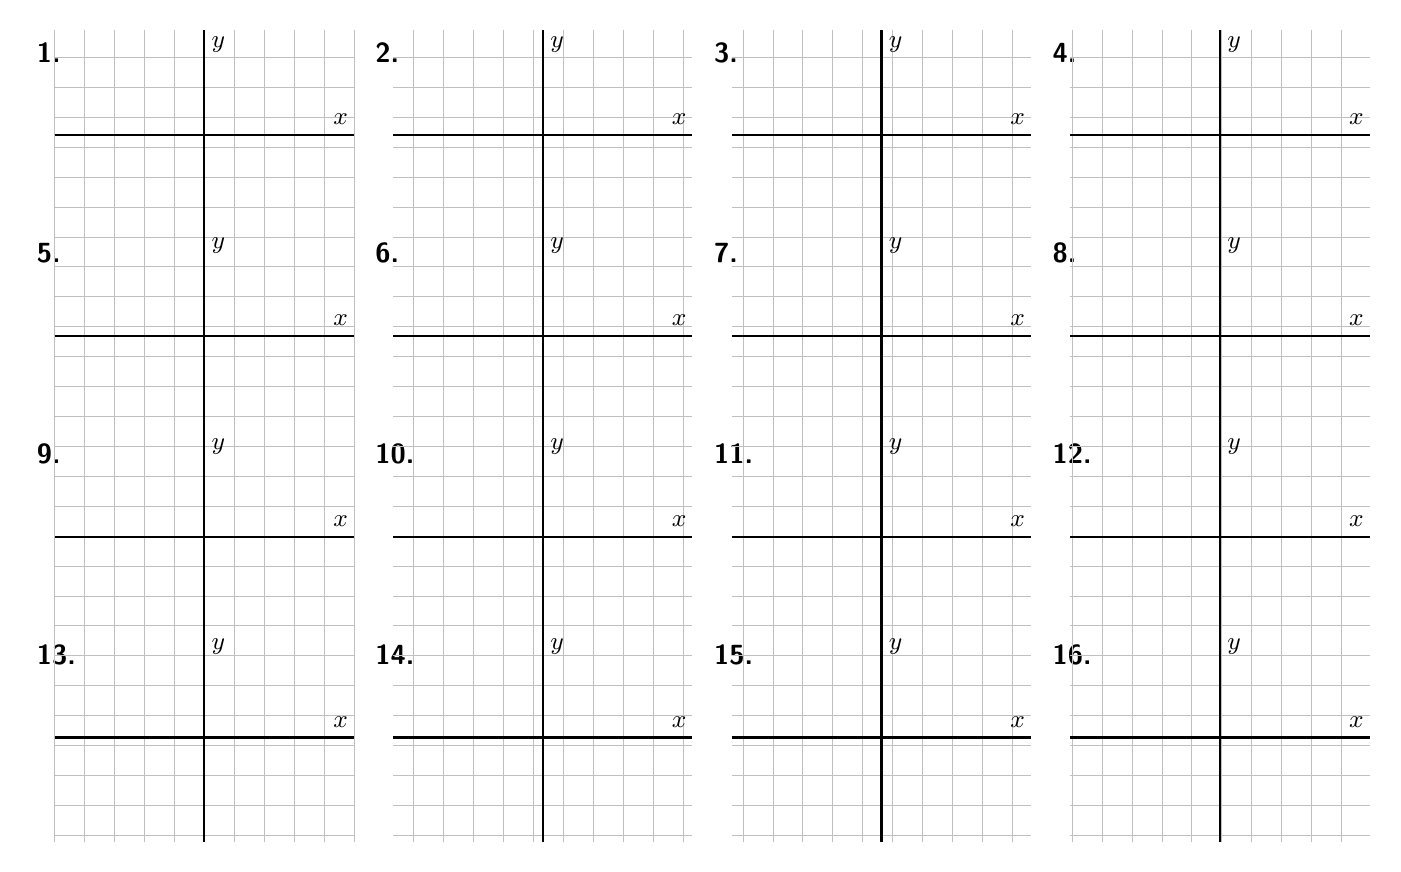
\begin{tikzpicture}[x=1cm,y=1cm]
\node[anchor=west,font=\bfseries] at (-0.35,12.98) {1.};
\draw[step=0.38cm,very thin,color=gray!50] (0.0,10.6) grid (3.8,13.26);
\draw[thick] (1.9,10.6) -- (1.9,13.26);
\draw[thick] (0.0,11.93) -- (3.8,11.93);
\node[font=\small] at (3.63,12.129999999999999) {$x$};
\node[font=\small] at (2.08,13.08) {$y$};
\node[anchor=west,font=\bfseries] at (3.9499999999999997,12.98) {2.};
\draw[step=0.38cm,very thin,color=gray!50] (4.3,10.6) grid (8.1,13.26);
\draw[thick] (6.199999999999999,10.6) -- (6.199999999999999,13.26);
\draw[thick] (4.3,11.93) -- (8.1,11.93);
\node[font=\small] at (7.93,12.129999999999999) {$x$};
\node[font=\small] at (6.38,13.08) {$y$};
\node[anchor=west,font=\bfseries] at (8.25,12.98) {3.};
\draw[step=0.38cm,very thin,color=gray!50] (8.6,10.6) grid (12.399999999999999,13.26);
\draw[thick] (10.5,10.6) -- (10.5,13.26);
\draw[thick] (8.6,11.93) -- (12.399999999999999,11.93);
\node[font=\small] at (12.23,12.129999999999999) {$x$};
\node[font=\small] at (10.68,13.08) {$y$};
\node[anchor=west,font=\bfseries] at (12.55,12.98) {4.};
\draw[step=0.38cm,very thin,color=gray!50] (12.9,10.6) grid (16.7,13.26);
\draw[thick] (14.8,10.6) -- (14.8,13.26);
\draw[thick] (12.9,11.93) -- (16.7,11.93);
\node[font=\small] at (16.53,12.129999999999999) {$x$};
\node[font=\small] at (14.98,13.08) {$y$};
\node[anchor=west,font=\bfseries] at (-0.35,10.43) {5.};
\draw[step=0.38cm,very thin,color=gray!50] (0.0,8.05) grid (3.8,10.71);
\draw[thick] (1.9,8.05) -- (1.9,10.71);
\draw[thick] (0.0,9.38) -- (3.8,9.38);
\node[font=\small] at (3.63,9.58) {$x$};
\node[font=\small] at (2.08,10.530000000000001) {$y$};
\node[anchor=west,font=\bfseries] at (3.9499999999999997,10.43) {6.};
\draw[step=0.38cm,very thin,color=gray!50] (4.3,8.05) grid (8.1,10.71);
\draw[thick] (6.199999999999999,8.05) -- (6.199999999999999,10.71);
\draw[thick] (4.3,9.38) -- (8.1,9.38);
\node[font=\small] at (7.93,9.58) {$x$};
\node[font=\small] at (6.38,10.530000000000001) {$y$};
\node[anchor=west,font=\bfseries] at (8.25,10.43) {7.};
\draw[step=0.38cm,very thin,color=gray!50] (8.6,8.05) grid (12.399999999999999,10.71);
\draw[thick] (10.5,8.05) -- (10.5,10.71);
\draw[thick] (8.6,9.38) -- (12.399999999999999,9.38);
\node[font=\small] at (12.23,9.58) {$x$};
\node[font=\small] at (10.68,10.530000000000001) {$y$};
\node[anchor=west,font=\bfseries] at (12.55,10.43) {8.};
\draw[step=0.38cm,very thin,color=gray!50] (12.9,8.05) grid (16.7,10.71);
\draw[thick] (14.8,8.05) -- (14.8,10.71);
\draw[thick] (12.9,9.38) -- (16.7,9.38);
\node[font=\small] at (16.53,9.58) {$x$};
\node[font=\small] at (14.98,10.530000000000001) {$y$};
\node[anchor=west,font=\bfseries] at (-0.35,7.88) {9.};
\draw[step=0.38cm,very thin,color=gray!50] (0.0,5.5) grid (3.8,8.16);
\draw[thick] (1.9,5.5) -- (1.9,8.16);
\draw[thick] (0.0,6.83) -- (3.8,6.83);
\node[font=\small] at (3.63,7.03) {$x$};
\node[font=\small] at (2.08,7.98) {$y$};
\node[anchor=west,font=\bfseries] at (3.9499999999999997,7.88) {10.};
\draw[step=0.38cm,very thin,color=gray!50] (4.3,5.5) grid (8.1,8.16);
\draw[thick] (6.199999999999999,5.5) -- (6.199999999999999,8.16);
\draw[thick] (4.3,6.83) -- (8.1,6.83);
\node[font=\small] at (7.93,7.03) {$x$};
\node[font=\small] at (6.38,7.98) {$y$};
\node[anchor=west,font=\bfseries] at (8.25,7.88) {11.};
\draw[step=0.38cm,very thin,color=gray!50] (8.6,5.5) grid (12.399999999999999,8.16);
\draw[thick] (10.5,5.5) -- (10.5,8.16);
\draw[thick] (8.6,6.83) -- (12.399999999999999,6.83);
\node[font=\small] at (12.23,7.03) {$x$};
\node[font=\small] at (10.68,7.98) {$y$};
\node[anchor=west,font=\bfseries] at (12.55,7.88) {12.};
\draw[step=0.38cm,very thin,color=gray!50] (12.9,5.5) grid (16.7,8.16);
\draw[thick] (14.8,5.5) -- (14.8,8.16);
\draw[thick] (12.9,6.83) -- (16.7,6.83);
\node[font=\small] at (16.53,7.03) {$x$};
\node[font=\small] at (14.98,7.98) {$y$};
\node[anchor=west,font=\bfseries] at (-0.35,5.33) {13.};
\draw[step=0.38cm,very thin,color=gray!50] (0.0,2.95) grid (3.8,5.61);
\draw[thick] (1.9,2.95) -- (1.9,5.61);
\draw[thick] (0.0,4.28) -- (3.8,4.28);
\node[font=\small] at (3.63,4.48) {$x$};
\node[font=\small] at (2.08,5.43) {$y$};
\node[anchor=west,font=\bfseries] at (3.9499999999999997,5.33) {14.};
\draw[step=0.38cm,very thin,color=gray!50] (4.3,2.95) grid (8.1,5.61);
\draw[thick] (6.199999999999999,2.95) -- (6.199999999999999,5.61);
\draw[thick] (4.3,4.28) -- (8.1,4.28);
\node[font=\small] at (7.93,4.48) {$x$};
\node[font=\small] at (6.38,5.43) {$y$};
\node[anchor=west,font=\bfseries] at (8.25,5.33) {15.};
\draw[step=0.38cm,very thin,color=gray!50] (8.6,2.95) grid (12.399999999999999,5.61);
\draw[thick] (10.5,2.95) -- (10.5,5.61);
\draw[thick] (8.6,4.28) -- (12.399999999999999,4.28);
\node[font=\small] at (12.23,4.48) {$x$};
\node[font=\small] at (10.68,5.43) {$y$};
\node[anchor=west,font=\bfseries] at (12.55,5.33) {16.};
\draw[step=0.38cm,very thin,color=gray!50] (12.9,2.95) grid (16.7,5.61);
\draw[thick] (14.8,2.95) -- (14.8,5.61);
\draw[thick] (12.9,4.28) -- (16.7,4.28);
\node[font=\small] at (16.53,4.48) {$x$};
\node[font=\small] at (14.98,5.43) {$y$};
\end{tikzpicture}
\end{center}
\settasks{label=\textbf{\arabic*.}, label-width=2.2em, item-indent=2.95em, column-sep=1.3cm, after-item-skip=0.75em}
\begin{tasks}(2)
\task Draw \mbox{$ y=(x-3)^2-4 $}. Label the turning point and the axis of symmetry.
\task Draw \mbox{$ y=-2(x+1)^2+5 $}. Label the turning point and the axis of symmetry.
\task Draw \mbox{$ y=\frac{1}{2}(x-4)^2-3 $}. Label the turning point and the axis of symmetry.
\task Draw \mbox{$ y=x^2-8x+12 $}. Label the turning point and the axis of symmetry.
\task Draw \mbox{$ y=-x^2+6x-5 $}. Label the turning point and the axis of symmetry.
\task Draw \mbox{$ y=2x^2+4x-6 $}. Label the turning point and the axis of symmetry.
\task Draw \mbox{$ y=\frac{1}{2}x^2-3x+2 $}. Label the turning point and the axis of symmetry.
\task Draw \mbox{$ y=-\frac{1}{2}x^2-2x+3 $}. Label the turning point and the axis of symmetry.
\task Draw \mbox{$ y=(x+2)^2-1 $}. Also mark where it crosses the $x$-axis.
\task Draw \mbox{$ y=-(x-4)^2+2 $}. Also mark where it crosses the $x$-axis.
\task Draw \mbox{$ y=x^2+2x-8 $}. Also mark where it crosses the $x$-axis.
\task Draw \mbox{$ y=-x^2+4x-1 $}. Also mark where it crosses the $x$-axis.
\task Draw \mbox{$ y=2(x-2)^2+1 $}. Choose a sensible table, then draw it.
\task Draw \mbox{$ y=-2(x+3)^2+4 $}. Choose a sensible table, then draw it.
\task Draw \mbox{$ y=\frac{1}{2}(x+1)^2-4 $}. Choose a sensible table, then draw it.
\task Draw \mbox{$ y=x^2-10x+21 $}. Choose a sensible table, then draw it.
\end{tasks}
\end{document}
